\documentclass[border=6pt]{standalone}
\usepackage[T1]{fontenc}
\usepackage[utf8]{inputenc}
\usepackage[scaled=0.98]{helvet}
\renewcommand{\familydefault}{\sfdefault}
\usepackage{amsmath}
\usepackage{graphicx}
\graphicspath{{../../../../../../exercises_lecturenotes/lecture_notes/kurs100_lektionsnoter/}}
\usepackage{tikz}
\usepackage{pgfplots}
\pgfplotsset{compat=1.18}
\usetikzlibrary{arrows.meta, decorations.pathreplacing, calc, positioning, fit, backgrounds, shapes.geometric}
\usepgfplotslibrary{groupplots,fillbetween}
\definecolor{scanpink}{HTML}{E5006D}
\definecolor{scanteal}{HTML}{00A6A6}
\definecolor{scannavy}{HTML}{243746}
\definecolor{scanlightgray}{HTML}{F1F2F3}
    \definecolor{scanrateNavy}{HTML}{17365D}
    \definecolor{scanrateTeal}{HTML}{2A8C82}
    \definecolor{scanrateGold}{HTML}{D8A23A}
\definecolor{scanrateNavy}{HTML}{17365D}
\definecolor{scanrateTeal}{HTML}{2A8C82}
\definecolor{scanrateGold}{HTML}{D8A23A}
\definecolor{scanrateLight}{HTML}{EEF5F4}
\begin{document}
    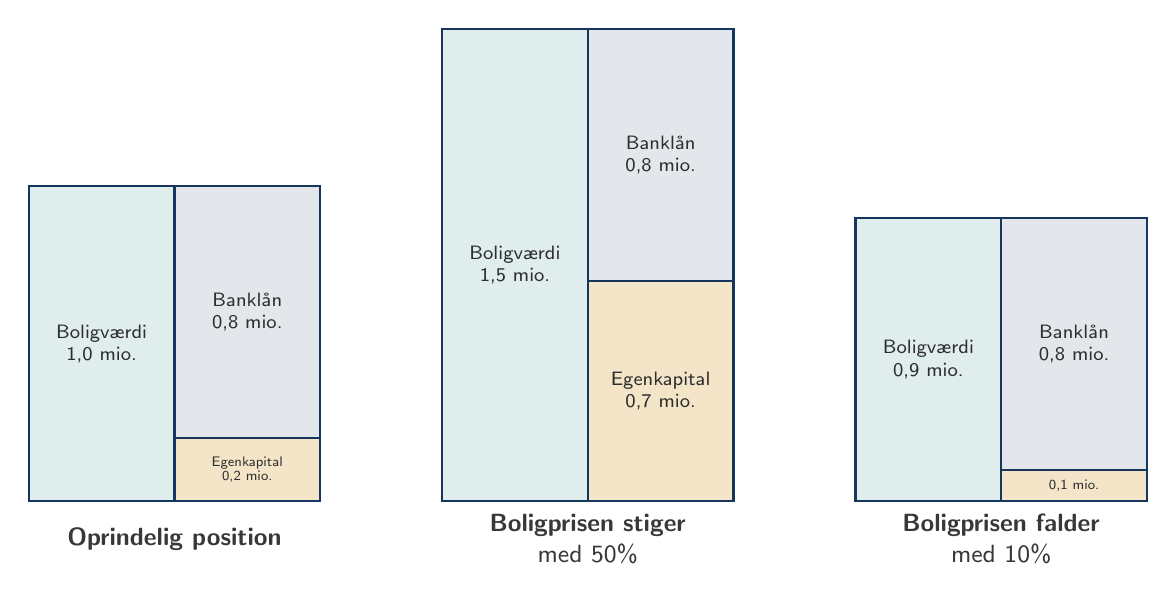
\begin{tikzpicture}[
        font=\small,
        balancebox/.style={
            draw=scanrateNavy,
            line width=0.8pt
        },
        assetbox/.style={
            balancebox,
            fill=scanrateTeal!15
        },
        debtbox/.style={
            balancebox,
            fill=scanrateNavy!12
        },
        equitybox/.style={
            balancebox,
            fill=scanrateGold!28
        },
        boxlabel/.style={
            align=center,
            inner sep=1.5pt,
            font=\scriptsize,
            text width=1.75cm,
            text=black!82
        },
        scenariolabel/.style={
            align=center,
            text=black!78
        }
    ]

    % Den lodrette skala er 4 cm pr. mio. USD.
    % Balancerne er bundjusterede, så højderne kan sammenlignes direkte.

    \begin{scope}[xshift=-5.25cm]
        \path[assetbox] (-1.85,0) rectangle (0,4.00);
        \path[equitybox] (0,0) rectangle (1.85,0.80);
        \path[debtbox] (0,0.80) rectangle (1.85,4.00);

        \node[boxlabel] at (-0.925,2.00) {Boligværdi\\1,0~mio.};
        \node[boxlabel] at (0.925,2.40) {Banklån\\0,8~mio.};
        \node[boxlabel,font=\tiny] at (0.925,0.40)
            {Egenkapital\\[-1pt]0,2~mio.};
        \node[scenariolabel] at (0,-0.48)
            {\textbf{Oprindelig position}};
    \end{scope}

    \begin{scope}
        \path[assetbox] (-1.85,0) rectangle (0,6.00);
        \path[equitybox] (0,0) rectangle (1.85,2.80);
        \path[debtbox] (0,2.80) rectangle (1.85,6.00);

        \node[boxlabel] at (-0.925,3.00) {Boligværdi\\1,5~mio.};
        \node[boxlabel] at (0.925,4.40) {Banklån\\0,8~mio.};
        \node[boxlabel] at (0.925,1.40) {Egenkapital\\0,7~mio.};
        \node[scenariolabel] at (0,-0.48)
            {\textbf{Boligprisen stiger}\\med 50\%};
    \end{scope}

    \begin{scope}[xshift=5.25cm]
        \path[assetbox] (-1.85,0) rectangle (0,3.60);
        \path[equitybox] (0,0) rectangle (1.85,0.40);
        \path[debtbox] (0,0.40) rectangle (1.85,3.60);

        \node[boxlabel] at (-0.925,1.80) {Boligværdi\\0,9~mio.};
        \node[boxlabel] at (0.925,2.00) {Banklån\\0,8~mio.};
        \node[boxlabel,font=\tiny] at (0.925,0.20) {0,1~mio.};
        \node[scenariolabel] at (0,-0.48)
            {\textbf{Boligprisen falder}\\med 10\%};
    \end{scope}

    \end{tikzpicture}
\end{document}
